\documentclass[aspectratio=169,17pt,fleqn]{beamer}

\usetheme{Madrid}
\usecolortheme{dolphin}
\setbeamertemplate{navigation symbols}{}
\setbeamertemplate{footline}[frame number]

\usepackage{amsmath,amssymb,array}
% \setmathfont{Latin Modern Math}

\usepackage{fontspec}      % text fonts (beamer uses sans by default)
\usepackage{unicode-math}  % modern math

\AtBeginSection[]{
  \begin{frame}
    \centering
    \vfill
    \Large\insertsectionhead
    \vfill
  \end{frame}
}

\usepackage{tikz}
\usetikzlibrary{positioning,matrix}


\title{Interpretations for $n$-ary relations}
\author{PHI~201 -- Introductory Logic}
\date{November 10, 2025}

\begin{document}

\frame{\titlepage}

\begin{frame}{ }

  How do we know that there isn't a valid proof with lines like this?

  \bigskip \begin{tabular}{>{\raggedleft\arraybackslash}p{1.5cm} >{\centering\arraybackslash}p{1.0cm} p{5cm} >{\raggedright\arraybackslash}p{3.5cm}}
    1 & (1) & $\forall x\exists yRxy$ & A \\
      & $\vdots$ & \\
    1 & (n) & $\exists y\forall xRxy$ & 
\end{tabular}

\end{frame}

\begin{frame}

  What kind of thing in the universe of sets should be the
  interpretation of an $n$-ary relation symbol?


\end{frame}

\begin{frame}

  We say that $A\times B$ is a \textbf{Cartesian product} of sets $A$
  and $B$ just in case: elements of $A\times B$ are in one-to-one
  correspondence with pairs of elements from $A$ and $B$.

  \bigskip We can represent elements of $A\times B$ as ordered pairs:
  $\{ \langle a,b\rangle \mid a\in A,b\in B\}$.

  \bigskip $\langle a,b\rangle = \langle c,d\rangle$ iff $a=c$ and
  $b=d$.

\end{frame}

\begin{frame}{Example of Cartesian product}

Let \(A = \{1, 2, 3\}\) and \(B = \{\alpha, \beta\}\).

\bigskip $A \times B = \{(1,\alpha), (1,\beta), (2,\alpha), (2,\beta), (3,\alpha), (3,\beta)\}.$

\bigskip Since \(|A| = 3\) and \(|B| = 2\), we have \(|A \times B| = 3 \times 2 = 6.\)

\end{frame}

\begin{frame}{Cartesian Product and the Plane \(\mathbb{R}^2\)}

\small 


\begin{center}
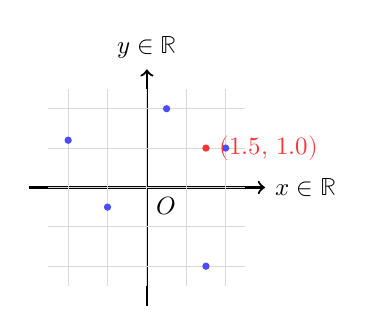
\begin{tikzpicture}[scale=0.5, every node/.style={font=\small}]
  % Axes
  \draw[->, thick] (-3,0) -- (3,0) node[right] {$x \in \mathbb{R}$};
  \draw[->, thick] (0,-3) -- (0,3) node[above] {$y \in \mathbb{R}$};
  
  % Grid
  \draw[gray!30] (-2.5,-2.5) grid (2.5,2.5);
  
  % Points
  \foreach \x/\y in {-2/1.2, -1/-0.5, 0.5/2, 1.5/-2, 2/1}{
    \filldraw[blue!70] (\x,\y) circle (2.2pt);
  }
  
  % Highlighted point
  \filldraw[red!80] (1.5,1.0) circle (2.2pt);
  \node[anchor=west, red!80] at (1.6,1.0) {$(1.5,\,1.0)$};
  
  % Origin
  \node[below right] at (0,0) {$O$};
\end{tikzpicture}
\end{center}

\vspace{0.5em}

\begin{itemize}
\item The Cartesian product \(\mathbb{R} \times \mathbb{R}\) forms the
  \textbf{Euclidean plane}.
  \item Each point corresponds to a unique ordered pair \((x,y)\).
  \item This idea generalizes to \(\mathbb{R}^3, \mathbb{R}^4,\) and
    beyond.
\end{itemize}

\end{frame}

\begin{frame}

  \begin{itemize}  
  \item The \textbf{extension} of a relation on a set $A$ is a subset
    of the set $A\times A$ of ordered pairs.
  \item Example: The extension of the relation ``$x$ is legally
    married to $y$ in the US'' is the set of all pairs of people who
    are legally married in the US.
  \end{itemize}

\end{frame}

\begin{frame}{Test your understanding}

  \begin{itemize}
  \item What is the extension of $x\neq y$ as a relation on the
    natural numbers?
  \item What is the extension of $x=y$ as a relation on the natural
    numbers?
  \item $x\neq x$ is not a relation, it's a predicate.
  \end{itemize}

\end{frame}

\begin{frame}{Test your understanding}

  \begin{itemize}
  \item What is the extension of the relation $y=2x+1$ on the real
    numbers?
  \item What is the extension of the relation
    \[ (y=2x+1)\wedge (x^2+y^2=1) \] on the real numbers?
  \end{itemize}

\end{frame}

\begin{frame}

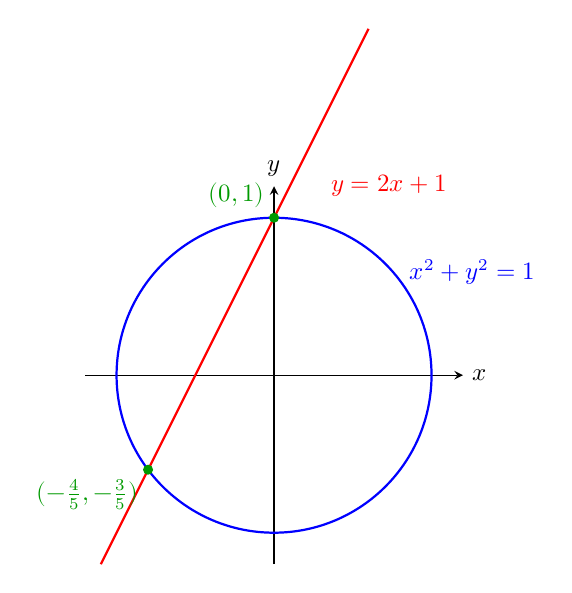
\begin{tikzpicture}[scale=2, >=stealth, every node/.style={font=\small}]
  % Axes
  \draw[->] (-1.2,0) -- (1.2,0) node[right] {$x$};
  \draw[->] (0,-1.2) -- (0,1.2) node[above] {$y$};

  % Circle x^2 + y^2 = 1
  \draw[blue, thick] (0,0) circle (1);
  \node[blue, below right] at (0.8,0.8) {$x^2 + y^2 = 1$};

  % Line y = 2x + 1
  \draw[red, thick, domain=-1.1:0.6, smooth, variable=\x]
    plot ({\x}, {2*\x + 1});
  \node[red, right] at (0.3,1.2) {$y = 2x + 1$};

  % Intersection points
  \filldraw[green!60!black] (0,1) circle (0.8pt)
    node[above left] {$(0,1)$};
  \filldraw[green!60!black] (-0.8,-0.6) circle (0.8pt)
    node[below left] {$(-\tfrac{4}{5},-\tfrac{3}{5})$};

\end{tikzpicture}

\end{frame}

\begin{frame}{Worked problem}

  Show that $\exists x\exists yRxy$ does not logically imply
  $\exists xRxx$.

  \vspace{6em}


\end{frame}

\section{Discovering and presenting interpretations}

\begin{frame}

  \begin{itemize}
  \item With more experience, you get to know structures that can be
    used as interpretations.
  \item In many cases, it will suffice to work with a small number of
    nodes in a graph-like structure.
  \end{itemize}

\end{frame}


\begin{frame}{Worked example}

  $ \forall x\forall y(Rxy\to Ryx) $

  \vspace{6em}



\end{frame}

\begin{frame}{The decision problem}

  \begin{itemize}
  \item If the task is to decide whether a \textbf{propositional}
    sequent is valid, then there is a \textbf{algorithm} that settles
    the question.
  \item Princeton's own Alonzo Church, along with his student Alan
    Turing, proved that there is no such algorithm for logic with
    relation symbols.
    \begin{itemize}
    \item Most interesting mathematical theories, e.g.\ arithmetic,
      set theory, are undecidable.
    \end{itemize}
  \end{itemize}



\end{frame}

\begin{frame}{What this means for you}

  \begin{itemize}
  \item I cannot teach you a procedure that will always find a model
    if a sentence is consistent (or a counterexample if a sequent is
    invalid).
  \item But I can give you a tour of the infinite universe of
    structures that could serve as counterexamples.
  \end{itemize}

\end{frame}

\begin{frame}{Worked example}

  $\forall x\forall y\exists z(Rxz\wedge Ryz)$

  \small 

  \bigskip Domain: $\{ a,b\}$, $R$: $\{ \langle a,b\rangle ,\langle b,b\rangle
  \} $

  \medskip Extension of $(Rxz \wedge Ryz)$: $\{\, \langle a,a,b\rangle,\
  \langle a,b,b\rangle,\ \langle b,a,b\rangle,\ \langle b,b,b\rangle
  \,\}$

  \medskip Extension of $\exists z (Rxz \wedge Ryz)$:
  $\{\, \langle a,a\rangle,\ \langle a,b\rangle,\ \langle b,a\rangle,\
  \langle b,b\rangle \,\}$



\end{frame}


\begin{frame}{Example}

  What is the extension of $\exists y Rxy$?

  \bigskip \begin{tabular}{cc}

  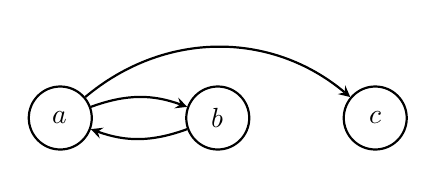
\begin{tikzpicture}[>=stealth, node distance=2cm, thick]
  % Nodes
  \node[circle, draw, minimum size=8mm] (a) {$a$};
  \node[circle, draw, minimum size=8mm, right of=a] (b) {$b$};
  \node[circle, draw, minimum size=8mm, right of=b] (c) {$c$};

  % Relation arrows (Rxy)
  \draw[->] (a) to[bend left=20] node[above] {} (b);
  \draw[->] (a) to[bend left=40] node[above] {} (c);
  \draw[->] (b) to[bend left=20] node[below] {} (a);

\end{tikzpicture}

    & \[
\begin{array}{c||c|c|c}
Rxy & a & b & c \\ \hline\hline
a &   & \checkmark & \checkmark \\ \hline
b & \checkmark &   &   \\ \hline
c &   &   &   
\end{array}
\]

\text{Rows $a,b$ satisfy } \exists y\,Rxy. \end{tabular}
  
  


\end{frame}




\end{document}

%%% Local Variables:
%%% mode: latex
%%% TeX-master: t
%%% End:
